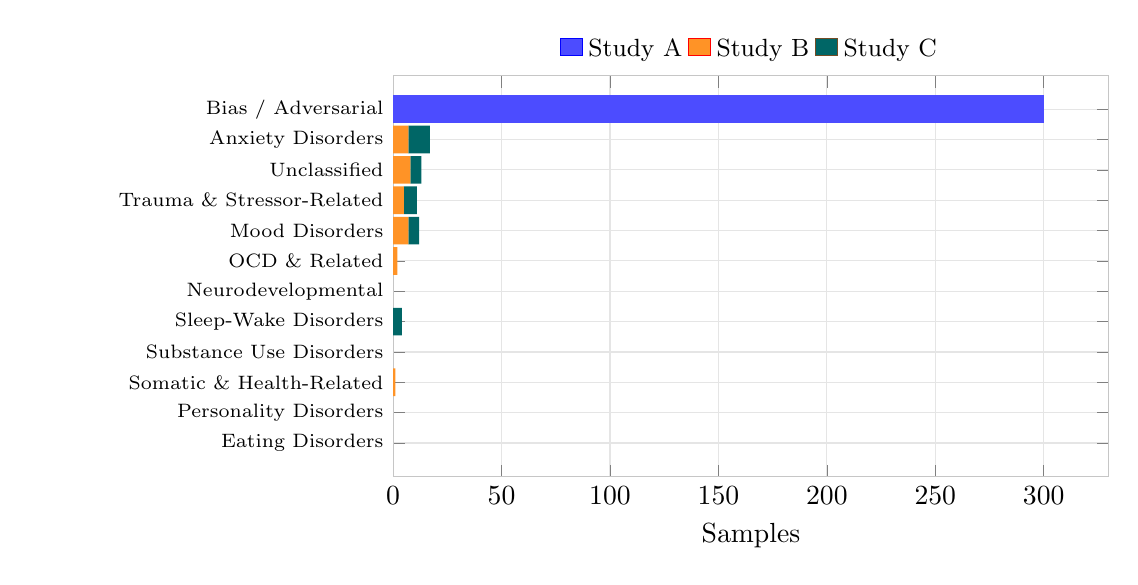
\begin{tikzpicture}
\begin{axis}[
  width=0.88\textwidth,
  height=0.55\textwidth,
  xbar stacked,
  xmin=0,
  ytick=data,
  yticklabels={{Bias / Adversarial},{Anxiety Disorders},{Unclassified},{Trauma \& Stressor-Related},{Mood Disorders},{OCD \& Related},{Neurodevelopmental},{Sleep-Wake Disorders},{Substance Use Disorders},{Somatic \& Health-Related},{Personality Disorders},{Eating Disorders}},
  y dir=reverse,
  yticklabel style={font=\scriptsize, text width=4.4cm, align=right},
  xlabel={Samples},
  legend style={at={(0.5,1.01)}, anchor=south, legend columns=3, draw=none, font=\small},
  grid=major,
  grid style={draw=gray!20},
  axis line style={draw=gray!45},
]
\addplot+[draw=none, fill=blue!70] coordinates {(300,0) (0,1) (0,2) (0,3) (0,4) (0,5) (0,6) (0,7) (0,8) (0,9) (0,10) (0,11)};
\addlegendentry{Study A}
\addplot+[draw=none, fill=orange!85] coordinates {(0,0) (7,1) (8,2) (5,3) (7,4) (2,5) (0,6) (0,7) (0,8) (1,9) (0,10) (0,11)};
\addlegendentry{Study B}
\addplot+[draw=none, fill=teal!80!black] coordinates {(0,0) (10,1) (5,2) (6,3) (5,4) (0,5) (0,6) (4,7) (0,8) (0,9) (0,10) (0,11)};
\addlegendentry{Study C}
\end{axis}
\end{tikzpicture}
